\documentclass{article}
\usepackage[utf8]{inputenc}

\title{Support Vector Machines}
\author{Sylesh Suresh}
\date{October 2017}

\usepackage{natbib}
\usepackage{graphicx}
\usepackage{amsmath}
\usepackage{bm}

\begin{document}

\maketitle

\section{Introduction}
Support Vector Machines (SVMs) are one of the most popular supervised learning models today, able to perform both linear and nonlinear classification.
\section{Linear Classification}
The idea behind SVMs is to maximize the margin, the distance between the hyperplane (decision boundary) and the samples nearest to this hyperplane, called support vectors. 
\begin{figure}[h!]
\centering
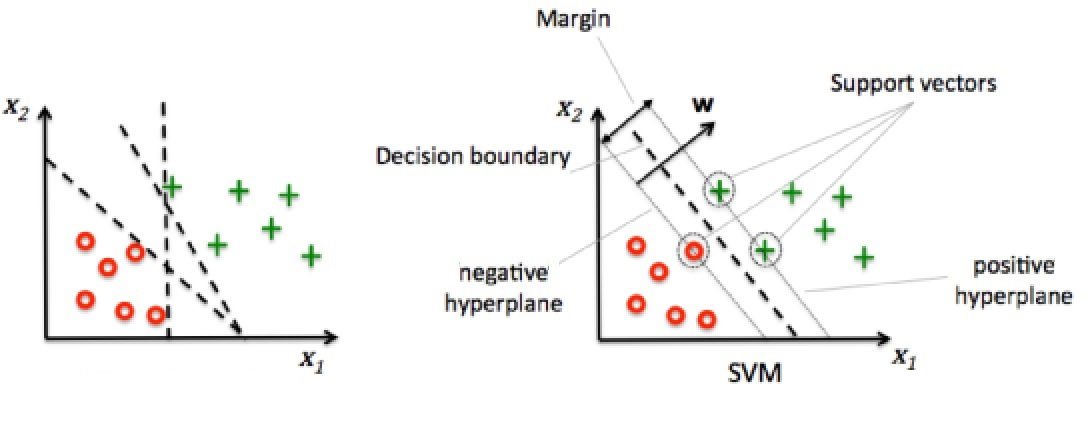
\includegraphics[scale=0.4]{svm.jpg}
\caption{Support Vector Machine}
\label{fig:svm}
\end{figure}
The decision boundaries to the left separate the training data correctly but would not generalize well to unseen data, being too close to the training samples (i.e. having a small margin). On the other hand, the decision boundary to the right marked by the dashed line separates the training data and generalizes well to unseen data, having a large margin. Maximization of the margin allows for the least generalization error.

$\bm{w}$ is defined as a vector normal to the decision boundary. 
The positive hyperplane is defined as
\[ \bm{w \cdot x_{pos}} + w_0 = 1 \]
while the negative hyperplane is:
\[ \bm{w \cdot x_{neg}} + w_0 = -1 \]

We can combine these equations by subtracting the second equation from the first:
\begin{equation} \label{eq:hyperplanes}
\bm{w}{(x_{pos} - x_{neg})} = 2 
\end{equation}

To calculate the margin, first, let us take the difference between a positive support vector and a negative support vector.

\[ x_{pos} - x_{neg} \]

Then, we need to multiply this by a unit vector perpendicular to the hyperplanes. We earlier defined $\bm{w}$ to be normal to the hyperplanes, so $\frac{\bm{w}}{||\bm{w}||}$ serves this purpose:

\[ \frac{\bm{w}(x_{pos} - x_{neg})}{||\bm{w}||} \]

Using ~\ref{eq:hyperplanes}, we arrive at:

\[ \frac{\bm{w}(x_{pos} - x_{neg})}{||\bm{w}||} = \frac{2}{||\bm{w}||} \]


We must maximize $\frac{2}{||\bm{w}||}$ to maximize the margin. For mathematical convenience, we can minimize $\frac{1}{2}{||\bm{w}||^2}$ to achieve the same effect. The constraint for this optimization problem is that the samples are actually classified correctly:

\[ \bm{w \cdot x_{i}} + w_0 \geq 1 \text{ if $y_i = 1$} \]

\[ \bm{w \cdot x_{i}} + w_0 < -1 \text{ if $y_i = -1$}\]

where $x_i$ is a particular sample and $y_i$ is the class of the sample. More compactly:

\[ y_i(w_0 + \bm{w \cdot x_i}) \geq 1 \]

After maximizing the margin, our decision rule is:

\[ y_i = sign(\bm{w \cdot x_i} + w_0) \]

That is, points to the left of the decision boundary are classified as negative while points to the right are classified as positive.

\section{Nonlinear Classification using Kernels}

In the real world, data is usually not linearly separable, meaning that the support vector machine as cannot accurately separate the data. However, we can project the data onto a higher dimensional space where the data is linearly separable using a mapping function $\phi{(\cdot)}$ For example:
\[ \phi{(x_1, x_2)} = (z_1, z_2, z_3) = (x_1, x_2, x_1^2 + x_2^2) \]
Using this mapping function allows us to separate the two classes below (indicated by red and blue) with a linear hyperplane. We can then project this back into two-dimensional space where the decision boundary becomes nonlinear.

\begin{figure}[h!]
\centering
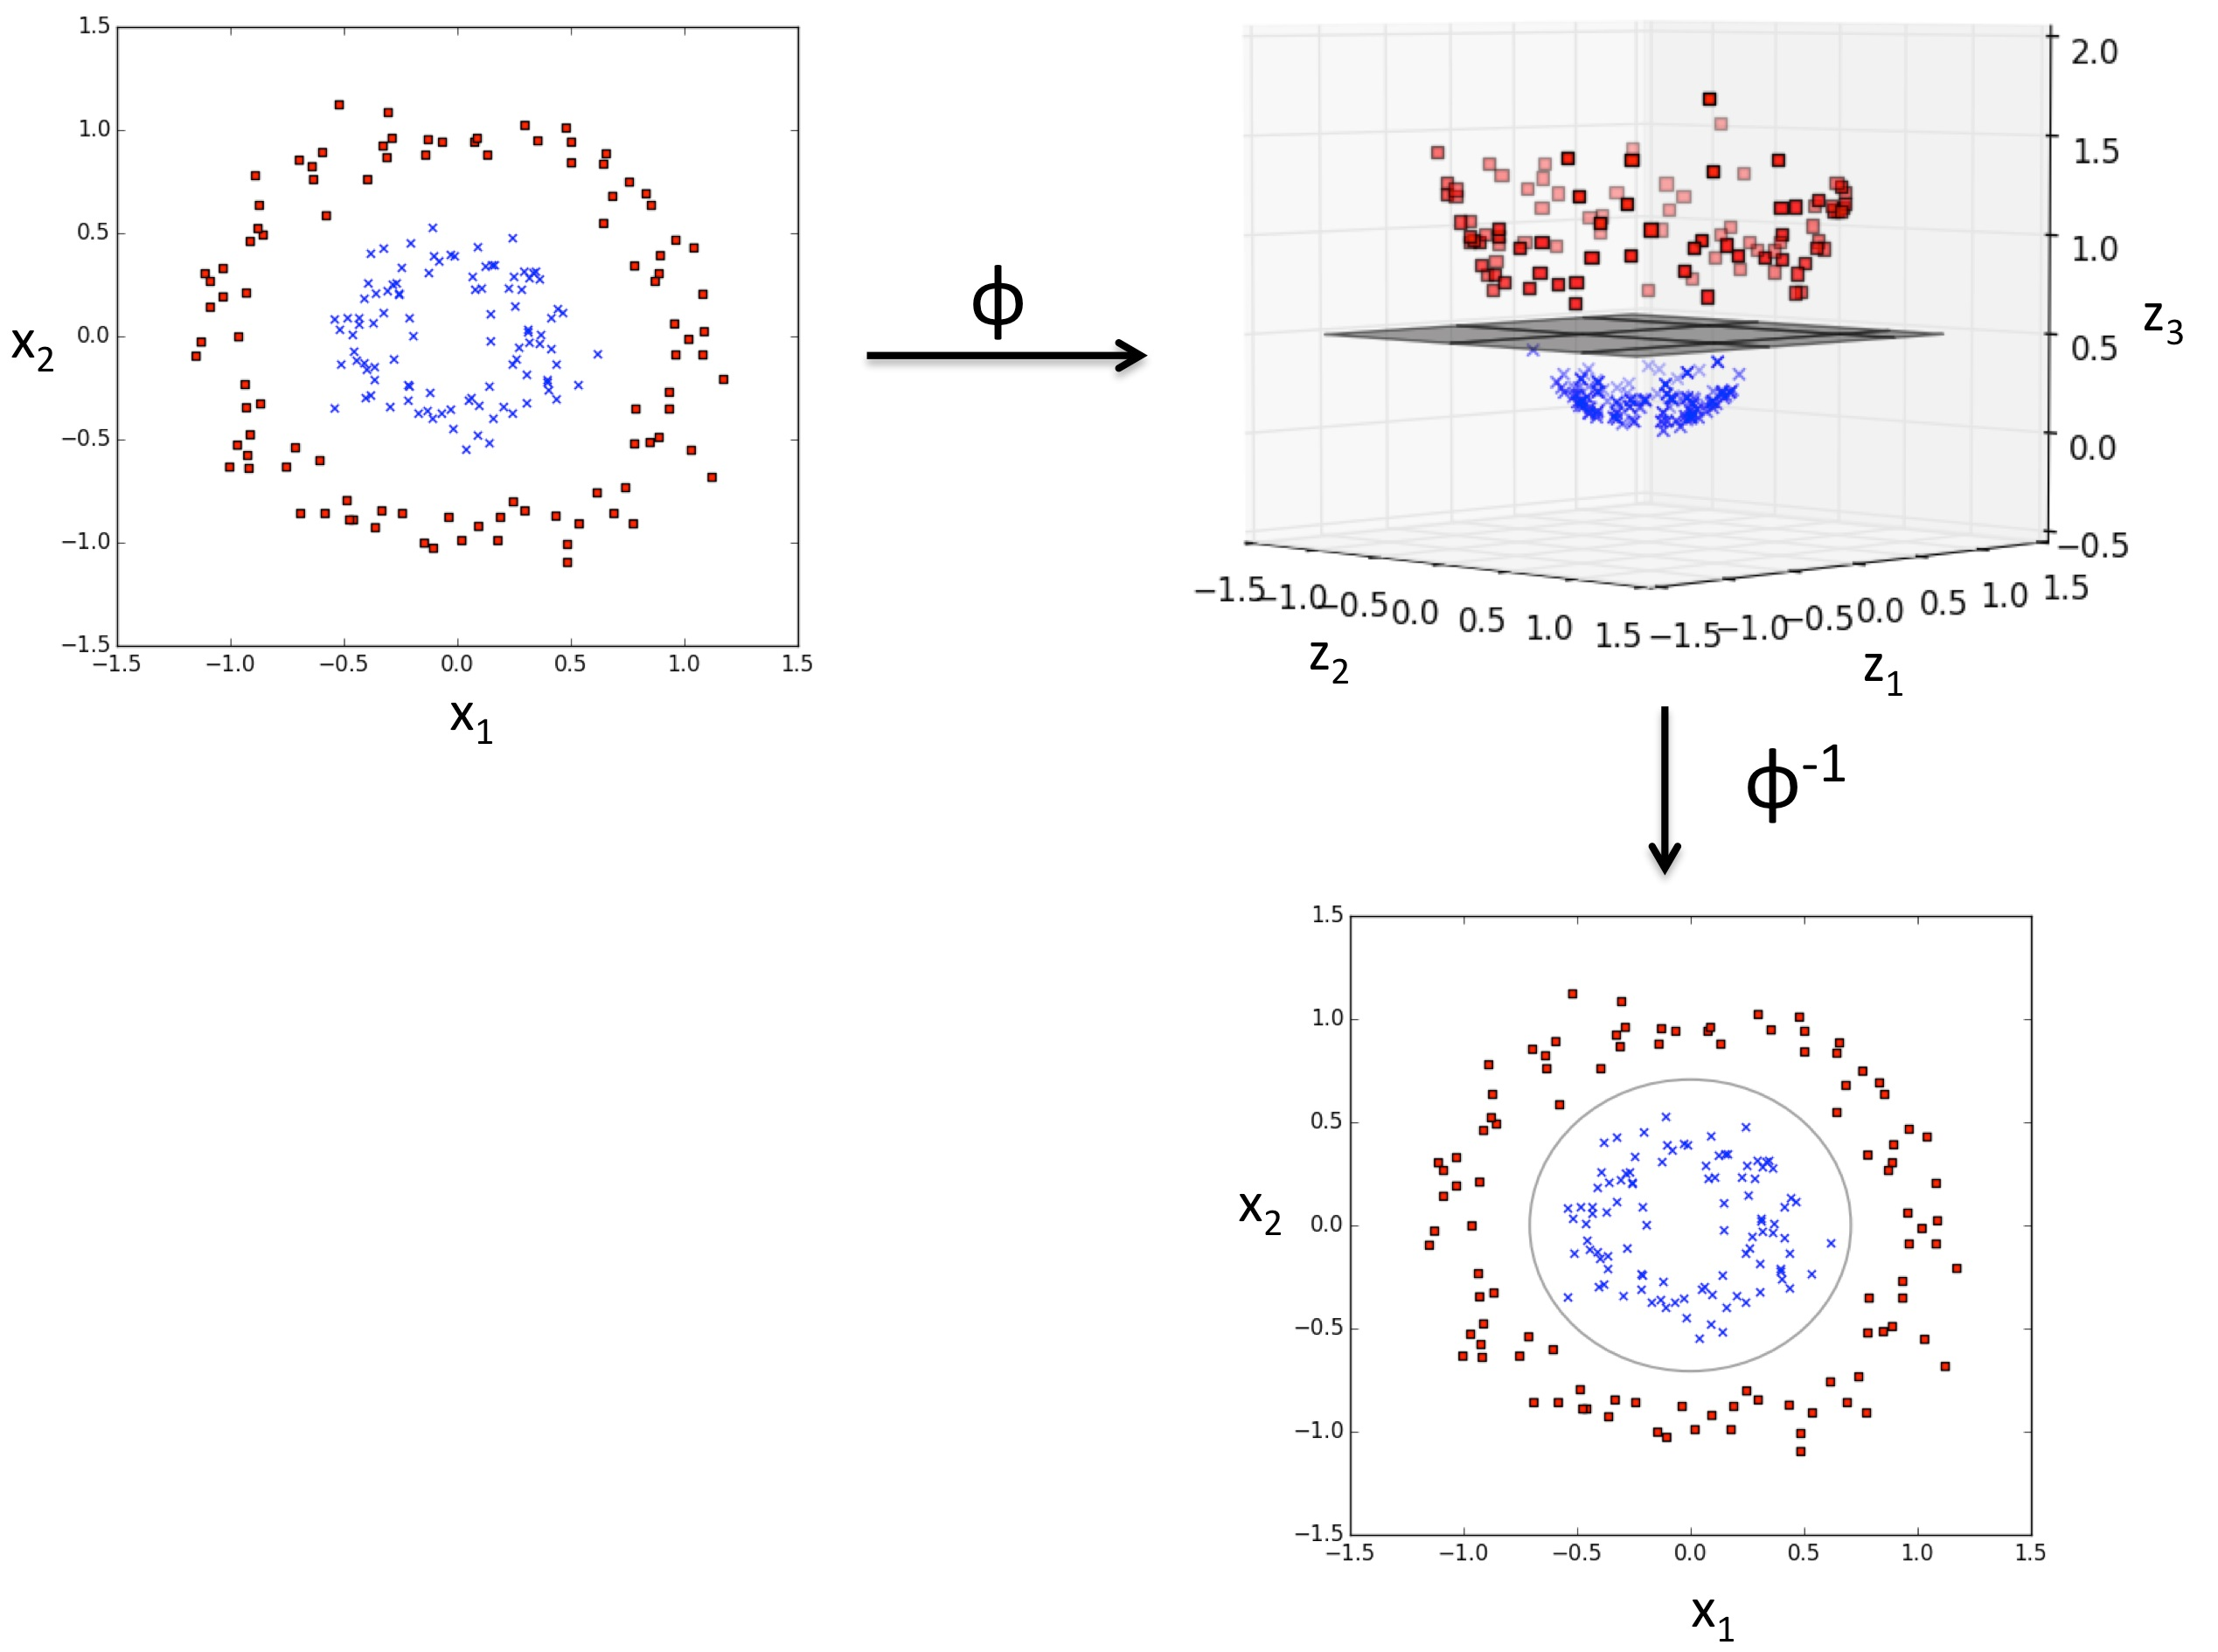
\includegraphics[scale=0.18]{dimensions.jpg}
\caption{Projecting to higher space}
\label{fig:mapping}
\end{figure}
The problem, however, with this approach is its efficiency. When solving the optimization problem of maximizing the margin, the pair-wise dot products of different training samples $\bm{x_i}$ and $\bm{x_j}$ must be calculated, a very computationally expensive process in high-dimensional space. To solve this, we can use the kernel trick; we can use kernel functions to implicitly calculate the dot product of $\bm{x_i}$ and $\bm{x_j}$ without explicitly projecting them into higher dimensional space. 

One of the most popular kernel functions is the Radial Basis Function kernel (RBF kernel) or Gaussian kernel:

\[ k(\bm{x_i}, \bm{x_j}) = \exp{(-\gamma||\bm{x_i}-\bm{x_j}||^2}) \]

$\gamma$ is a free parameter that can be optimized.

\end{document}
